\documentclass[border=12pt]{standalone}
\usepackage{tikz}
\usepackage{pgfplots}
\usepackage{amsmath,amssymb}
\usepackage[T1]{fontenc}
\usepackage{lmodern}
\usepackage{xcolor}
\usetikzlibrary{arrows.meta,positioning,shapes.geometric,calc,fit,matrix,backgrounds}
\pgfplotsset{compat=1.18}
\definecolor{ink}{HTML}{17202A}
\definecolor{blue}{HTML}{2463EB}
\definecolor{bluefill}{HTML}{EDF3FF}
\definecolor{green}{HTML}{16804A}
\definecolor{greenfill}{HTML}{EAF7EF}
\definecolor{amber}{HTML}{B56800}
\definecolor{amberfill}{HTML}{FFF4D8}
\definecolor{red}{HTML}{B42318}
\definecolor{redfill}{HTML}{FDEDEC}
\definecolor{purple}{HTML}{6B46C1}
\definecolor{purplefill}{HTML}{F2EDFF}
\definecolor{gray}{HTML}{667085}
\definecolor{light}{HTML}{F4F6F8}
\definecolor{linegray}{HTML}{CBD2D9}
\tikzset{
  every node/.style={font=\sffamily},
  box/.style={draw=ink, rounded corners=3pt, line width=1.1pt, fill=white, align=center, inner xsep=9pt, inner ysep=7pt, font=\sffamily\small},
  bluebox/.style={box, fill=bluefill, draw=blue},
  greenbox/.style={box, fill=greenfill, draw=green},
  amberbox/.style={box, fill=amberfill, draw=amber},
  redbox/.style={box, fill=redfill, draw=red},
  purplebox/.style={box, fill=purplefill, draw=purple},
  ghost/.style={box, draw=linegray, fill=light, text=gray},
  title/.style={font=\sffamily\bfseries\Large, text=ink, align=center},
  subtitle/.style={font=\sffamily\small, text=gray, align=center},
  arrow/.style={-{Latex[length=3mm,width=2mm]}, line width=1.2pt, draw=ink},
  bluearrow/.style={-{Latex[length=3mm,width=2mm]}, line width=1.2pt, draw=blue},
  greenarrow/.style={-{Latex[length=3mm,width=2mm]}, line width=1.2pt, draw=green},
  redarrow/.style={-{Latex[length=3mm,width=2mm]}, line width=1.2pt, draw=red},
  dashedarrow/.style={-{Latex[length=3mm,width=2mm]}, line width=1pt, dashed, draw=gray},
  smalllabel/.style={font=\sffamily\scriptsize, text=gray, align=center},
}

\begin{document}
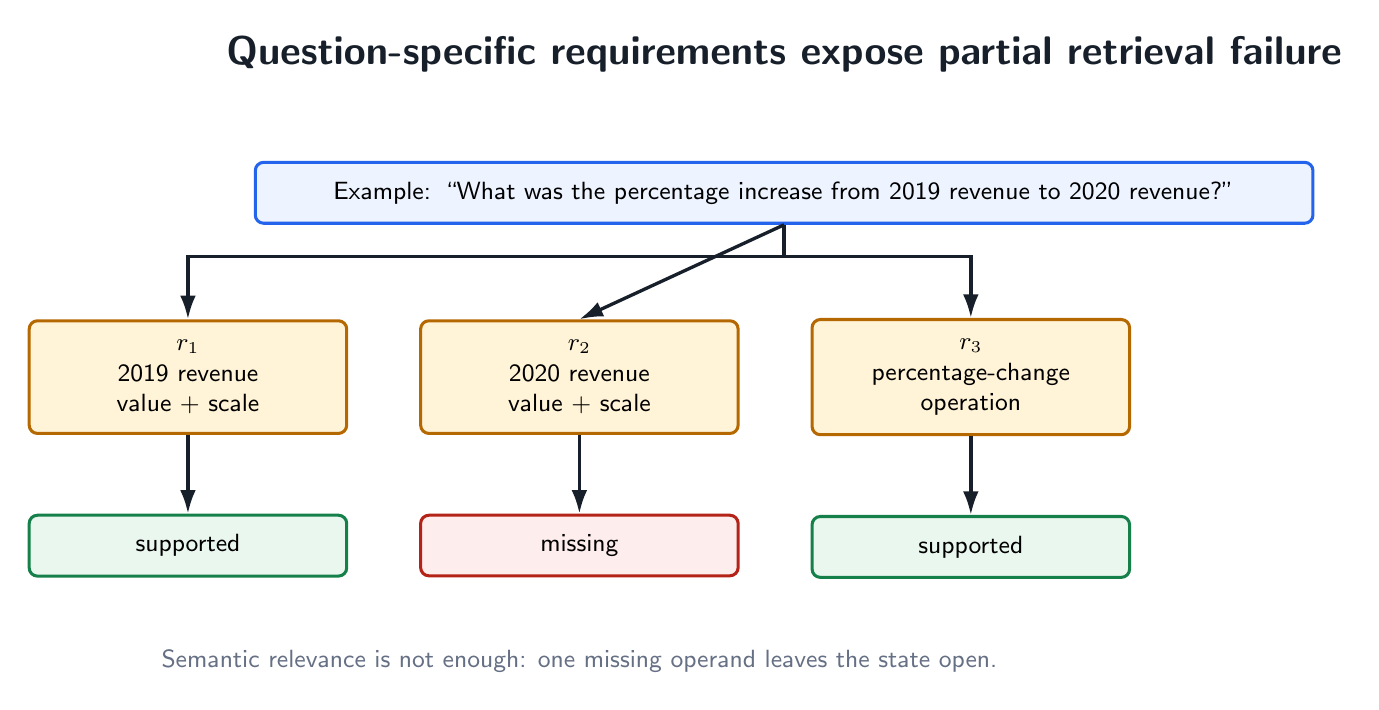
\begin{tikzpicture}[node distance=8mm and 10mm]
\node[title] (t) {Question-specific requirements expose partial retrieval failure};
\node[bluebox, below=10mm of t, text width=12.8cm] (q) {Example: ``What was the percentage increase from 2019 revenue to 2020 revenue?''};
\node[amberbox, below left=12mm and -1.2cm of q, text width=3.4cm] (r1) {$r_1$\\2019 revenue\\value + scale};
\node[amberbox, right=9mm of r1, text width=3.4cm] (r2) {$r_2$\\2020 revenue\\value + scale};
\node[amberbox, right=9mm of r2, text width=3.4cm] (r3) {$r_3$\\percentage-change\\operation};
\node[greenbox, below=10mm of r1, text width=3.4cm] (s1) {supported};
\node[redbox, below=10mm of r2, text width=3.4cm] (s2) {missing};
\node[greenbox, below=10mm of r3, text width=3.4cm] (s3) {supported};
\draw[arrow](q.south)--++(0,-4mm)-|(r1.north); \draw[arrow](q.south)--(r2.north); \draw[arrow](q.south)--++(0,-4mm)-|(r3.north);
\draw[arrow](r1)--(s1);\draw[arrow](r2)--(s2);\draw[arrow](r3)--(s3);
\node[subtitle, below=8mm of s2] {Semantic relevance is not enough: one missing operand leaves the state open.};
\end{tikzpicture}
\end{document}
